% Options for packages loaded elsewhere
\PassOptionsToPackage{unicode}{hyperref}
\PassOptionsToPackage{hyphens}{url}
%
\documentclass[
]{article}
\usepackage{amsmath,amssymb}
\usepackage{iftex}
\ifPDFTeX
  \usepackage[T1]{fontenc}
  \usepackage[utf8]{inputenc}
  \usepackage{textcomp} % provide euro and other symbols
\else % if luatex or xetex
  \usepackage{unicode-math} % this also loads fontspec
  \defaultfontfeatures{Scale=MatchLowercase}
  \defaultfontfeatures[\rmfamily]{Ligatures=TeX,Scale=1}
\fi
\usepackage{lmodern}
\ifPDFTeX\else
  % xetex/luatex font selection
\fi
% Use upquote if available, for straight quotes in verbatim environments
\IfFileExists{upquote.sty}{\usepackage{upquote}}{}
\IfFileExists{microtype.sty}{% use microtype if available
  \usepackage[]{microtype}
  \UseMicrotypeSet[protrusion]{basicmath} % disable protrusion for tt fonts
}{}
\makeatletter
\@ifundefined{KOMAClassName}{% if non-KOMA class
  \IfFileExists{parskip.sty}{%
    \usepackage{parskip}
  }{% else
    \setlength{\parindent}{0pt}
    \setlength{\parskip}{6pt plus 2pt minus 1pt}}
}{% if KOMA class
  \KOMAoptions{parskip=half}}
\makeatother
\usepackage{xcolor}
\usepackage[margin=1in]{geometry}
\usepackage{color}
\usepackage{fancyvrb}
\newcommand{\VerbBar}{|}
\newcommand{\VERB}{\Verb[commandchars=\\\{\}]}
\DefineVerbatimEnvironment{Highlighting}{Verbatim}{commandchars=\\\{\}}
% Add ',fontsize=\small' for more characters per line
\usepackage{framed}
\definecolor{shadecolor}{RGB}{248,248,248}
\newenvironment{Shaded}{\begin{snugshade}}{\end{snugshade}}
\newcommand{\AlertTok}[1]{\textcolor[rgb]{0.94,0.16,0.16}{#1}}
\newcommand{\AnnotationTok}[1]{\textcolor[rgb]{0.56,0.35,0.01}{\textbf{\textit{#1}}}}
\newcommand{\AttributeTok}[1]{\textcolor[rgb]{0.13,0.29,0.53}{#1}}
\newcommand{\BaseNTok}[1]{\textcolor[rgb]{0.00,0.00,0.81}{#1}}
\newcommand{\BuiltInTok}[1]{#1}
\newcommand{\CharTok}[1]{\textcolor[rgb]{0.31,0.60,0.02}{#1}}
\newcommand{\CommentTok}[1]{\textcolor[rgb]{0.56,0.35,0.01}{\textit{#1}}}
\newcommand{\CommentVarTok}[1]{\textcolor[rgb]{0.56,0.35,0.01}{\textbf{\textit{#1}}}}
\newcommand{\ConstantTok}[1]{\textcolor[rgb]{0.56,0.35,0.01}{#1}}
\newcommand{\ControlFlowTok}[1]{\textcolor[rgb]{0.13,0.29,0.53}{\textbf{#1}}}
\newcommand{\DataTypeTok}[1]{\textcolor[rgb]{0.13,0.29,0.53}{#1}}
\newcommand{\DecValTok}[1]{\textcolor[rgb]{0.00,0.00,0.81}{#1}}
\newcommand{\DocumentationTok}[1]{\textcolor[rgb]{0.56,0.35,0.01}{\textbf{\textit{#1}}}}
\newcommand{\ErrorTok}[1]{\textcolor[rgb]{0.64,0.00,0.00}{\textbf{#1}}}
\newcommand{\ExtensionTok}[1]{#1}
\newcommand{\FloatTok}[1]{\textcolor[rgb]{0.00,0.00,0.81}{#1}}
\newcommand{\FunctionTok}[1]{\textcolor[rgb]{0.13,0.29,0.53}{\textbf{#1}}}
\newcommand{\ImportTok}[1]{#1}
\newcommand{\InformationTok}[1]{\textcolor[rgb]{0.56,0.35,0.01}{\textbf{\textit{#1}}}}
\newcommand{\KeywordTok}[1]{\textcolor[rgb]{0.13,0.29,0.53}{\textbf{#1}}}
\newcommand{\NormalTok}[1]{#1}
\newcommand{\OperatorTok}[1]{\textcolor[rgb]{0.81,0.36,0.00}{\textbf{#1}}}
\newcommand{\OtherTok}[1]{\textcolor[rgb]{0.56,0.35,0.01}{#1}}
\newcommand{\PreprocessorTok}[1]{\textcolor[rgb]{0.56,0.35,0.01}{\textit{#1}}}
\newcommand{\RegionMarkerTok}[1]{#1}
\newcommand{\SpecialCharTok}[1]{\textcolor[rgb]{0.81,0.36,0.00}{\textbf{#1}}}
\newcommand{\SpecialStringTok}[1]{\textcolor[rgb]{0.31,0.60,0.02}{#1}}
\newcommand{\StringTok}[1]{\textcolor[rgb]{0.31,0.60,0.02}{#1}}
\newcommand{\VariableTok}[1]{\textcolor[rgb]{0.00,0.00,0.00}{#1}}
\newcommand{\VerbatimStringTok}[1]{\textcolor[rgb]{0.31,0.60,0.02}{#1}}
\newcommand{\WarningTok}[1]{\textcolor[rgb]{0.56,0.35,0.01}{\textbf{\textit{#1}}}}
\usepackage{graphicx}
\makeatletter
\def\maxwidth{\ifdim\Gin@nat@width>\linewidth\linewidth\else\Gin@nat@width\fi}
\def\maxheight{\ifdim\Gin@nat@height>\textheight\textheight\else\Gin@nat@height\fi}
\makeatother
% Scale images if necessary, so that they will not overflow the page
% margins by default, and it is still possible to overwrite the defaults
% using explicit options in \includegraphics[width, height, ...]{}
\setkeys{Gin}{width=\maxwidth,height=\maxheight,keepaspectratio}
% Set default figure placement to htbp
\makeatletter
\def\fps@figure{htbp}
\makeatother
\setlength{\emergencystretch}{3em} % prevent overfull lines
\providecommand{\tightlist}{%
  \setlength{\itemsep}{0pt}\setlength{\parskip}{0pt}}
\setcounter{secnumdepth}{-\maxdimen} % remove section numbering
\ifLuaTeX
\usepackage[bidi=basic]{babel}
\else
\usepackage[bidi=default]{babel}
\fi
\babelprovide[main,import]{spanish}
% get rid of language-specific shorthands (see #6817):
\let\LanguageShortHands\languageshorthands
\def\languageshorthands#1{}
\usepackage{booktabs}
\usepackage{longtable}
\usepackage{array}
\usepackage{multirow}
\usepackage{wrapfig}
\usepackage{float}
\usepackage{colortbl}
\usepackage{pdflscape}
\usepackage{tabu}
\usepackage{threeparttable}
\usepackage{threeparttablex}
\usepackage[normalem]{ulem}
\usepackage{makecell}
\usepackage{xcolor}
\ifLuaTeX
  \usepackage{selnolig}  % disable illegal ligatures
\fi
\usepackage{bookmark}
\IfFileExists{xurl.sty}{\usepackage{xurl}}{} % add URL line breaks if available
\urlstyle{same}
\hypersetup{
  pdftitle={Decisión multicriterio: Elección de la mejora más óptima para su implementación en un equipo de Formula Student},
  pdfauthor={Laura Mayorgas del Castillo},
  pdflang={es},
  hidelinks,
  pdfcreator={LaTeX via pandoc}}

\title{Decisión multicriterio: Elección de la mejora más óptima para su
implementación en un equipo de Formula Student}
\author{Laura Mayorgas del Castillo}
\date{}

\begin{document}
\maketitle

{
\setcounter{tocdepth}{2}
\tableofcontents
}
\newpage

\section{Introducción}\label{introducciuxf3n}

La Formula Student es la competición más prestigiosa a nivel ingenieril
del mundo. Es por eso que los distintos equipos buscan continuamente
mejoras que optimicen el rendimiento de sus monoplazas. Sin embargo,
debido a los recursos limitados y múltiples amplio abanico de mejoras,
elegir la más adecuada es un desafío. Este trabajo propone un enfoque de
decisiones multicriterio para identificar la mejora óptima, evaluando
factores como el rendimiento, el costo y el peso.

\begin{figure}
\centering
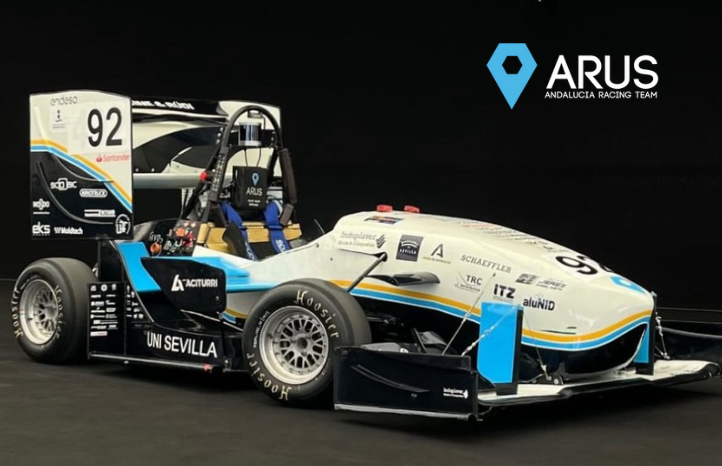
\includegraphics[width=4.16667in,height=\textheight]{Fotos/fotomonoplazas.png}
\caption{ART-24 D}
\end{figure}

ARUS es el equipo de Formula Student de la Universidad de Sevilla y del
cual vamos a realizar el trabajo.

\href{https://www.arusteam.com/}{\emph{(ARUS web)}}

\section{Criterios}\label{criterios}

Para la elección de la mejora más óptima tenemos que tener en cuanta
distintos criterios, en este caso los hemos resumidos en los siguientes
6.

\textbf{1. Peso Total del Monoplazas}

Este criterio afecta directamente en la aceleración y frenado del
monoplazas, además también tiene un impacto directo en el comportamiento
de este en las curvas. Es un criterio \textbf{\emph{desfavorable}} en el
sentido de que queremos mínimizar el peso.

\textbf{2. Coste de Fabricación}

Al tratarse de un equipo de universidad disponemos de un límite
presupuestario, por lo que siempre buscamos una opción económica y
asequible. También es un criterio en el que buscaremos el
\textbf{\emph{mínimo}}.

\textbf{3. Fiabilidad y Seguridad}

Valorar la robustez de la mejora propuesta y su impacto en la seguridad
del piloto, asegurando que el cambio no comprometa la durabilidad del
vehículo ni los estándares de seguridad, todo debe cumplir las reglas
que la competición de Alemania (FSG) determina.
\href{https://www.formulastudent.de/fileadmin/user_upload/all/2025/rules/FS-Rules_2025_v1.0.pdf}{\emph{(enlace
a la normativa)}}\emph{.}

\textbf{4. Innovación}

Este criterio considera el grado de creatividad y originalidad de la
mejora, su potencial para introducir tecnologías o conceptos innovadores
y la posibilidad de marcar la diferencia en la competición con un diseño
único y eficiente. Existe un premio específico para el equipo más
innovador de la temporada.

\textbf{5. Evaluación de riesgos}

Análisis de los riesgos técnicos y operativos asociados a la
implementación de las distintas mejoras. Se consideran posibles fallos o
problemas que puedan surgir, así como el impacto que podrían tener en el
rendimiento o la seguridad del vehículo. Se requiere establecer un plan
de gestión de riesgos para mitigar los efectos adversos y reducir la
probabilidad de problemas en competencia.

\textbf{6. Sostenibilidad}

La sostenibilidad es cada vez más importante en el mundo actual esto se
ve reflejado en la competición de Formula Student. Este criterio evalúa
el impacto ambiental de los materiales, procesos y recursos utilizados
para implementar las mejoras en estudio. Se priorizarán materiales
reciclables y técnicas de fabricación ecoeficientes, buscando reducir la
huella de carbono.

\newpage

\section{Mejoras}\label{mejoras}

Serán las alternativas que evaluaremos en cada uno de los criterios que
hemos mencionado anteriormente. Veamos estas de forma detallada.

\textbf{1. Monocasco}

Durante la temporada 24 y anteriormente en el equipo siempre se ha
realizado un meneplazas cuyo chasis era tubular.

\begin{figure}
\centering
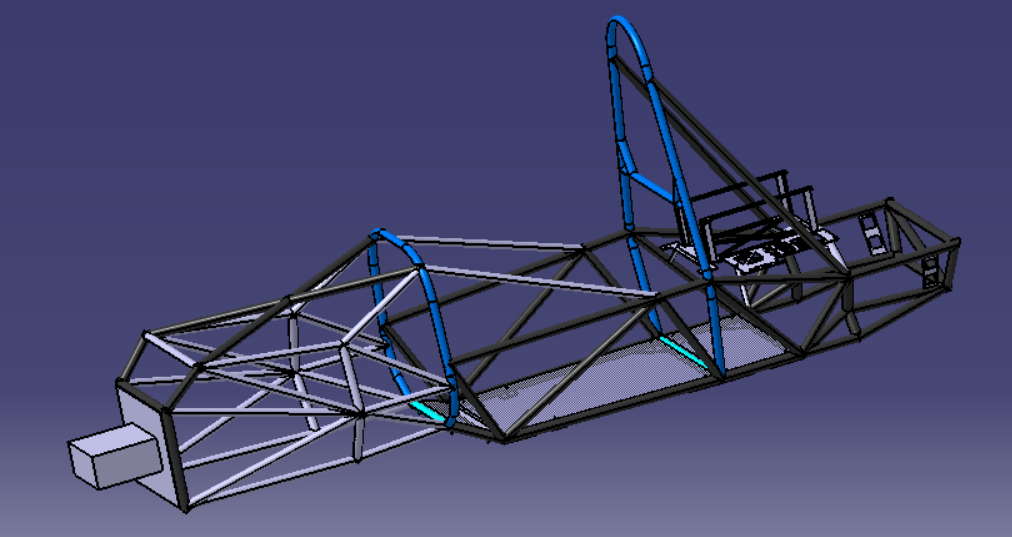
\includegraphics[width=4.16667in,height=\textheight]{Fotos/chasistubular.png}
\caption{ART-24 D Chasis Tubular}
\end{figure}

Consiste en una red de tubos de acero o aluminio soldados entre sí.

Se está planteando la opción de cambiar el diseño de este chasis a un
monocasco, siguiendo la tendencia adoptada por varios equipos de Formula
Student. Al adoptar un chasis monocasco, no solo reducimos
significativamente el peso del vehículo, sino que también incrementamos
la rigidez estructural, lo cual mejora el comportamiento dinámico del
mismo.

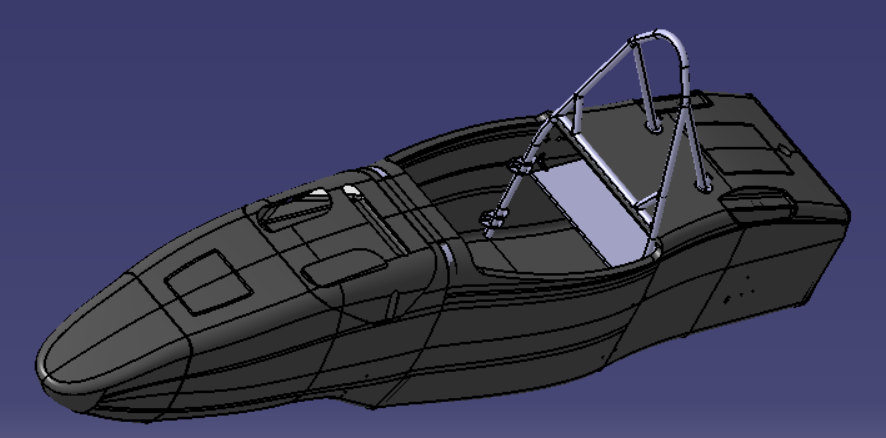
\includegraphics[width=4.16667in,height=\textheight]{Fotos/monocasco.png}
\newpage

\textbf{2. Tracción a las 4 rueda}

Conocido y llamado a partir de ahora como 4WD(4 Wheel Drive). Consiste
en lugar de tener un único motor, colocar uno en cada rueda. Este cambio
mejorará la aceleración, el control y la estabilidad en curvas al
distribuir la potencia en las cuatro ruedas, optimizando el agarre en
cualquier condición de pista.

\begin{figure}
\centering
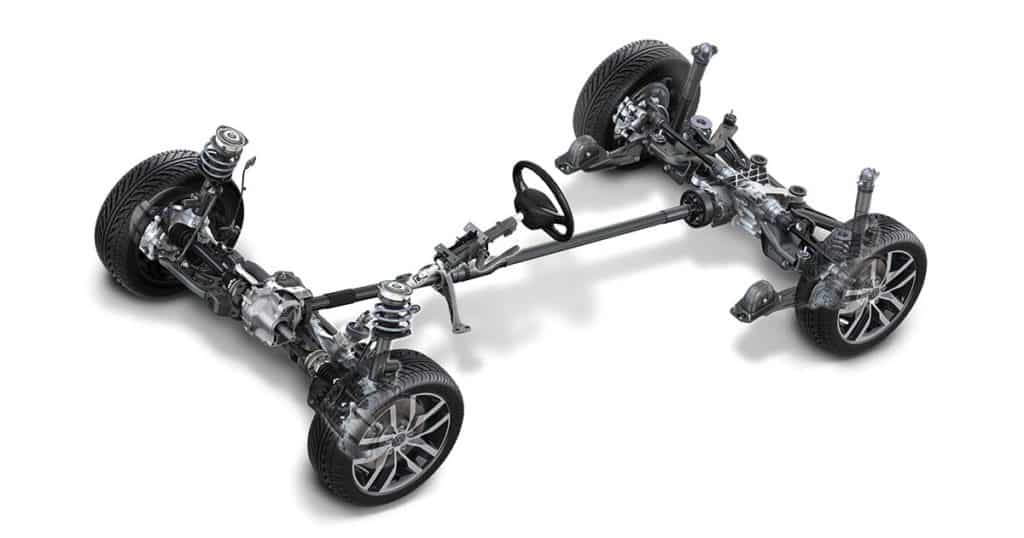
\includegraphics[width=4.16667in,height=\textheight]{Fotos/4WD.png}
\caption{Estructura de un 4WD}
\end{figure}

\textbf{3. Optimización de la batería}

Cambio de celdas, antes eran cilíndricas y se pretende pasar a las que
se pueden ver en la derecha, estas ocupan mucho menos sitio haciendo que
el computo general de la batería tenga un peso menor al de la temporada
de 2024. Además de un cambio en la configuración de la misma.

\begin{figure}
\centering
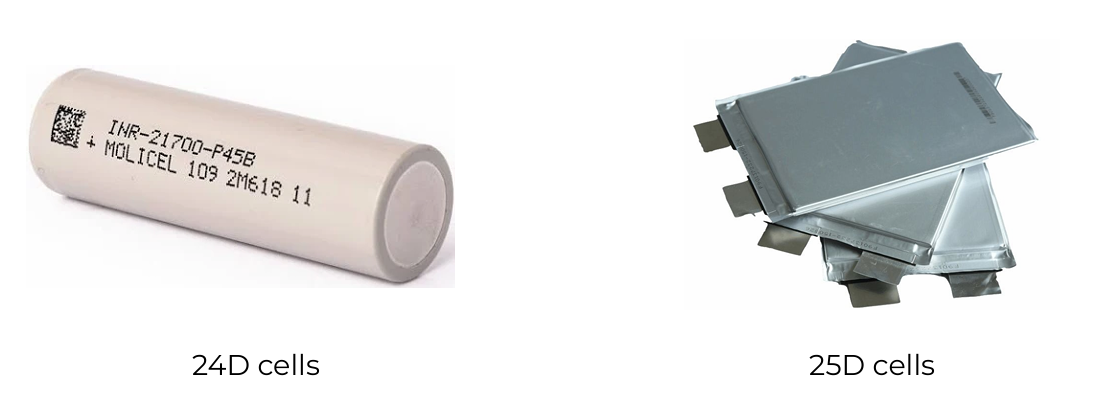
\includegraphics[width=4.16667in,height=\textheight]{Fotos/bateria.png}
\caption{Celdas batería}
\end{figure}

\textbf{4. Telemetría}

Sistema de monitorización en tiempo real que recolecta y transmite los
datos de los distintos componentes del vehículo hacia una estación
remota, permitiendo detectar posibles problemas en directo. Además de la
necesidad de conectar un sensor proporcionado por la misma competición
llamado \emph{dattalogger} que recoge todo estos datos.

\textbf{5. Diseño de Nuevas Aletas y Difusores para Aerodinámica} Busca
optimizar el flujo de aire alrededor del vehículo para mejorar el agarre
y la estabilidad. Este sistema se centra en controlar la distribución de
fuerzas aerodinámicas, aumentando la eficiencia y el rendimiento.

\newpage

\section{AHP}\label{ahp}

En primer lugar vamos a hacer una matriz que contenga la información al
comparar los distintos \textbf{\emph{criterios}}:

\begin{longtable}[t]{lrrrrrr}
\toprule
 & Peso & Coste & Fiabilidad & Innovación & Riesgo & Sostenibilidad\\
\midrule
\cellcolor{gray!10}{Peso} & \cellcolor{gray!10}{1.00} & \cellcolor{gray!10}{0.50} & \cellcolor{gray!10}{3.00} & \cellcolor{gray!10}{8} & \cellcolor{gray!10}{5.00} & \cellcolor{gray!10}{7.0}\\
Coste & 2.00 & 1.00 & 4.00 & 9 & 6.00 & 7.0\\
\cellcolor{gray!10}{Fiabilidad} & \cellcolor{gray!10}{0.33} & \cellcolor{gray!10}{0.25} & \cellcolor{gray!10}{1.00} & \cellcolor{gray!10}{4} & \cellcolor{gray!10}{2.00} & \cellcolor{gray!10}{4.0}\\
Innovación & 0.12 & 0.11 & 0.25 & 1 & 0.33 & 0.5\\
\cellcolor{gray!10}{Riesgo} & \cellcolor{gray!10}{0.20} & \cellcolor{gray!10}{0.17} & \cellcolor{gray!10}{0.50} & \cellcolor{gray!10}{3} & \cellcolor{gray!10}{1.00} & \cellcolor{gray!10}{2.0}\\
\addlinespace
Sostenibilidad & 0.14 & 0.14 & 0.25 & 2 & 0.50 & 1.0\\
\bottomrule
\end{longtable}

Ahora se hará una matriz para cada uno de los criterios haciendo
comparaciones dos a dos sobre las distintas alternativas yy ver cual es
preferible a cual, buscando simepre una estructura coherente y
respetando la relación de coherencia.

\begin{itemize}
\tightlist
\item
  \textbf{Peso Total del Monoplazas}
\end{itemize}

\begin{longtable}[t]{lrrrrr}
\toprule
 & Monocasco & 4WD & Batería & Telemetría & Aerodinámica\\
\midrule
\cellcolor{gray!10}{Monocasco} & \cellcolor{gray!10}{1.00} & \cellcolor{gray!10}{4.00} & \cellcolor{gray!10}{8.0} & \cellcolor{gray!10}{9} & \cellcolor{gray!10}{2.00}\\
4WD & 0.25 & 1.00 & 5.0 & 7 & 2.00\\
\cellcolor{gray!10}{Batería} & \cellcolor{gray!10}{0.12} & \cellcolor{gray!10}{0.20} & \cellcolor{gray!10}{1.0} & \cellcolor{gray!10}{2} & \cellcolor{gray!10}{0.25}\\
Telemetría & 0.11 & 0.14 & 0.5 & 1 & 0.17\\
\cellcolor{gray!10}{Aerodinámica} & \cellcolor{gray!10}{0.50} & \cellcolor{gray!10}{0.50} & \cellcolor{gray!10}{4.0} & \cellcolor{gray!10}{6} & \cellcolor{gray!10}{1.00}\\
\bottomrule
\end{longtable}

\begin{itemize}
\tightlist
\item
  \textbf{Coste de Fabricación}
\end{itemize}

\begin{longtable}[t]{lrrrrr}
\toprule
 & Monocasco & 4WD & Batería & Telemetría & Aerodinámica\\
\midrule
\cellcolor{gray!10}{Monocasco} & \cellcolor{gray!10}{1} & \cellcolor{gray!10}{0.5} & \cellcolor{gray!10}{0.11} & \cellcolor{gray!10}{0.14} & \cellcolor{gray!10}{0.2}\\
4WD & 2 & 1.0 & 0.17 & 0.33 & 1.0\\
\cellcolor{gray!10}{Batería} & \cellcolor{gray!10}{9} & \cellcolor{gray!10}{6.0} & \cellcolor{gray!10}{1.00} & \cellcolor{gray!10}{3.00} & \cellcolor{gray!10}{6.0}\\
Telemetría & 7 & 3.0 & 0.33 & 1.00 & 2.0\\
\cellcolor{gray!10}{Aerodinámica} & \cellcolor{gray!10}{5} & \cellcolor{gray!10}{1.0} & \cellcolor{gray!10}{0.17} & \cellcolor{gray!10}{0.50} & \cellcolor{gray!10}{1.0}\\
\bottomrule
\end{longtable}

\begin{itemize}
\tightlist
\item
  \textbf{Fiabilidad y seguridad}
\end{itemize}

\begin{longtable}[t]{lrrrrr}
\toprule
 & Monocasco & 4WD & Batería & Telemetría & Aerodinámica\\
\midrule
\cellcolor{gray!10}{Monocasco} & \cellcolor{gray!10}{1} & \cellcolor{gray!10}{0.14} & \cellcolor{gray!10}{0.2} & \cellcolor{gray!10}{0.11} & \cellcolor{gray!10}{0.5}\\
4WD & 7 & 1.00 & 2.0 & 0.50 & 7.0\\
\cellcolor{gray!10}{Batería} & \cellcolor{gray!10}{5} & \cellcolor{gray!10}{0.50} & \cellcolor{gray!10}{1.0} & \cellcolor{gray!10}{0.25} & \cellcolor{gray!10}{2.0}\\
Telemetría & 9 & 2.00 & 4.0 & 1.00 & 7.0\\
\cellcolor{gray!10}{Aerodinámica} & \cellcolor{gray!10}{2} & \cellcolor{gray!10}{0.14} & \cellcolor{gray!10}{0.5} & \cellcolor{gray!10}{0.14} & \cellcolor{gray!10}{1.0}\\
\bottomrule
\end{longtable}

\begin{itemize}
\tightlist
\item
  \textbf{Innovación}
\end{itemize}

\begin{longtable}[t]{lrrrrr}
\toprule
 & Monocasco & 4WD & Batería & Telemetría & Aerodinámica\\
\midrule
\cellcolor{gray!10}{Monocasco} & \cellcolor{gray!10}{1.00} & \cellcolor{gray!10}{5.0} & \cellcolor{gray!10}{5.0} & \cellcolor{gray!10}{2.00} & \cellcolor{gray!10}{9}\\
4WD & 0.20 & 1.0 & 1.0 & 0.33 & 5\\
\cellcolor{gray!10}{Batería} & \cellcolor{gray!10}{0.20} & \cellcolor{gray!10}{1.0} & \cellcolor{gray!10}{1.0} & \cellcolor{gray!10}{0.33} & \cellcolor{gray!10}{5}\\
Telemetría & 0.50 & 3.0 & 3.0 & 1.00 & 7\\
\cellcolor{gray!10}{Aerodinámica} & \cellcolor{gray!10}{0.11} & \cellcolor{gray!10}{0.2} & \cellcolor{gray!10}{0.2} & \cellcolor{gray!10}{0.14} & \cellcolor{gray!10}{1}\\
\bottomrule
\end{longtable}

\begin{itemize}
\tightlist
\item
  \textbf{Evaluación de riesgo}
\end{itemize}

\begin{longtable}[t]{lrrrrr}
\toprule
 & Monocasco & 4WD & Batería & Telemetría & Aerodinámica\\
\midrule
\cellcolor{gray!10}{Monocasco} & \cellcolor{gray!10}{1.00} & \cellcolor{gray!10}{0.5} & \cellcolor{gray!10}{0.20} & \cellcolor{gray!10}{0.14} & \cellcolor{gray!10}{3}\\
4WD & 2.00 & 1.0 & 0.33 & 0.17 & 5\\
\cellcolor{gray!10}{Batería} & \cellcolor{gray!10}{5.00} & \cellcolor{gray!10}{3.0} & \cellcolor{gray!10}{1.00} & \cellcolor{gray!10}{0.50} & \cellcolor{gray!10}{5}\\
Telemetría & 7.00 & 6.0 & 2.00 & 1.00 & 9\\
\cellcolor{gray!10}{Aerodinámica} & \cellcolor{gray!10}{0.33} & \cellcolor{gray!10}{0.2} & \cellcolor{gray!10}{0.20} & \cellcolor{gray!10}{0.11} & \cellcolor{gray!10}{1}\\
\bottomrule
\end{longtable}

\begin{itemize}
\tightlist
\item
  \textbf{Sostenibilidad}
\end{itemize}

\begin{longtable}[t]{lrrrrr}
\toprule
 & Monocasco & 4WD & Batería & Telemetría & Aerodinámica\\
\midrule
\cellcolor{gray!10}{Monocasco} & \cellcolor{gray!10}{1.0} & \cellcolor{gray!10}{0.50} & \cellcolor{gray!10}{2} & \cellcolor{gray!10}{0.17} & \cellcolor{gray!10}{0.33}\\
4WD & 2.0 & 1.00 & 3 & 0.20 & 0.33\\
\cellcolor{gray!10}{Batería} & \cellcolor{gray!10}{0.5} & \cellcolor{gray!10}{0.33} & \cellcolor{gray!10}{1} & \cellcolor{gray!10}{0.11} & \cellcolor{gray!10}{0.14}\\
Telemetría & 6.0 & 5.00 & 9 & 1.00 & 2.00\\
\cellcolor{gray!10}{Aerodinámica} & \cellcolor{gray!10}{3.0} & \cellcolor{gray!10}{3.00} & \cellcolor{gray!10}{7} & \cellcolor{gray!10}{0.50} & \cellcolor{gray!10}{1.00}\\
\bottomrule
\end{longtable}

\subsection{Mayor autovalor}\label{mayor-autovalor}

\textbf{Pesos locales}

\begin{Shaded}
\begin{Highlighting}[]
\NormalTok{wcriterios }\OtherTok{\textless{}{-}} \FunctionTok{multicriterio.metodoAHP.variante1.autovectormayorautovalor}\NormalTok{(tablacriterios)}
\NormalTok{wpeso }\OtherTok{\textless{}{-}} \FunctionTok{multicriterio.metodoAHP.variante1.autovectormayorautovalor}\NormalTok{(peso)}
\NormalTok{wcoste }\OtherTok{\textless{}{-}} \FunctionTok{multicriterio.metodoAHP.variante1.autovectormayorautovalor}\NormalTok{(coste)}
\NormalTok{wfiabilidad }\OtherTok{\textless{}{-}} \FunctionTok{multicriterio.metodoAHP.variante1.autovectormayorautovalor}\NormalTok{(fiabilidad)}
\NormalTok{winnovacion }\OtherTok{\textless{}{-}} \FunctionTok{multicriterio.metodoAHP.variante1.autovectormayorautovalor}\NormalTok{(innovacion)}
\NormalTok{wriesgo }\OtherTok{\textless{}{-}} \FunctionTok{multicriterio.metodoAHP.variante1.autovectormayorautovalor}\NormalTok{(riesgo)}
\NormalTok{wsostenibilidad }\OtherTok{\textless{}{-}} \FunctionTok{multicriterio.metodoAHP.variante1.autovectormayorautovalor}\NormalTok{(sostenibilidad)}
\end{Highlighting}
\end{Shaded}

\textbf{Pesos globales}

\begin{Shaded}
\begin{Highlighting}[]
\NormalTok{tabla1 }\OtherTok{\textless{}{-}} \FunctionTok{multicriterio.metodoAHP.pesosglobales\_entabla}\NormalTok{(wcriterios}\SpecialCharTok{$}\NormalTok{valoraciones.ahp, }
                                                       \FunctionTok{rbind}\NormalTok{(wpeso}\SpecialCharTok{$}\NormalTok{valoraciones.ahp,}
\NormalTok{                                                             wcoste}\SpecialCharTok{$}\NormalTok{valoraciones.ahp,}
\NormalTok{                                                             wfiabilidad}\SpecialCharTok{$}\NormalTok{valoraciones.ahp,}
\NormalTok{                                                             winnovacion}\SpecialCharTok{$}\NormalTok{valoraciones.ahp,}
\NormalTok{                                                             wriesgo}\SpecialCharTok{$}\NormalTok{valoraciones.ahp,}
\NormalTok{                                                             wsostenibilidad}\SpecialCharTok{$}\NormalTok{valoraciones.ahp))}
\end{Highlighting}
\end{Shaded}

\begin{verbatim}
## Warning in styling_latex_scale(out, table_info, "down"): Longtable cannot be
## resized.
\end{verbatim}

\begin{longtable}[t]{lrrrrrrr}
\toprule
 & Peso & Coste & Fiabilidad & Innovación & Riesgo & Sostenibilidad & Ponderadores Globales\\
\midrule
\cellcolor{gray!10}{Monocasco} & \cellcolor{gray!10}{0.4885995} & \cellcolor{gray!10}{0.0380167} & \cellcolor{gray!10}{0.0372497} & \cellcolor{gray!10}{0.4715277} & \cellcolor{gray!10}{0.0708690} & \cellcolor{gray!10}{0.0777909} & \cellcolor{gray!10}{0.1908290}\\
4WD & 0.2377226 & 0.0857595 & 0.2941296 & 0.1111723 & 0.1196405 & 0.1161993 & 0.1627871\\
\cellcolor{gray!10}{Batería} & \cellcolor{gray!10}{0.0532047} & \cellcolor{gray!10}{0.5361012} & \cellcolor{gray!10}{0.1398637} & \cellcolor{gray!10}{0.1111723} & \cellcolor{gray!10}{0.2733497} & \cellcolor{gray!10}{0.0421870} & \cellcolor{gray!10}{0.2849653}\\
Telemetría & 0.0345949 & 0.2249158 & 0.4670199 & 0.2733246 & 0.4986714 & 0.4876634 & 0.2329570\\
\cellcolor{gray!10}{Aerodinámica} & \cellcolor{gray!10}{0.1858782} & \cellcolor{gray!10}{0.1152067} & \cellcolor{gray!10}{0.0617371} & \cellcolor{gray!10}{0.0328030} & \cellcolor{gray!10}{0.0374694} & \cellcolor{gray!10}{0.2761594} & \cellcolor{gray!10}{0.1284616}\\
\addlinespace
Ponder.Criterios & 0.2993136 & 0.4203030 & 0.1287770 & 0.0318180 & 0.0740319 & 0.0457565 & NA\\
\bottomrule
\end{longtable}

\subsection{Media geométrica}\label{media-geomuxe9trica}

\end{document}
